\documentclass[a4paper,10pt]{article}
\usepackage[utf8]{inputenc}
\usepackage[english]{babel}
\usepackage{amsmath}
\usepackage{amsfonts}
\usepackage{amssymb}
\usepackage{graphicx}
\usepackage{wrapfig}

\usepackage{vmargin}
\setpapersize{A4}
\setmarginsrb{3cm}{3cm}{3cm}{3cm}%
{\baselineskip}{\baselineskip}{baselineskip}{\baselineskip}

\newcommand{\HRule}{\rule{\linewidth}{0.5mm}}
\setlength\parindent{0pt}
\setlength\parskip{0.3cm}

\title{FollowBot Android Application\\Project Pitch}
\author{Arian Stolwijk - 4001079\\Radu Florea - 4330358}
\date{}

\begin{document}

\maketitle

\section{Problem Description}

\begin{wrapfigure}{r}{0.4\textwidth}
  \vspace{-30pt}
  \begin{center}
    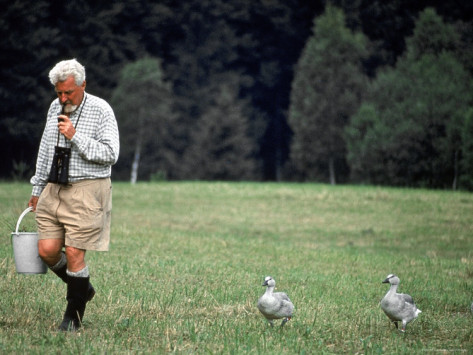
\includegraphics[width=0.38\textwidth]{geese.jpg}
    \vspace{-20pt}
  \end{center}
  \caption{Human followed by geese}
\label{fig:geese}
\end{wrapfigure}

There is an existing assumption that when baby geese come out of their eggs, they assume that their mother is the first
thing they see. Usually this is true, the baby geese following their mother until they able to fend for themselves. If a human were to be the first thing the baby geese saw, they would simply follow the human too, as seen in figure~\ref{fig:geese}.

Using an Android smartphone and a simple robot we can simulate the same effect. The smartphone acts as the mother (moved by the user) and the robot as the baby goose. The objective of the robot is to follow the smartphone and, thus, the person carrying it. This kind of behavior can be used to great effect in moving very heavy loads over long distances, eliminating the need to constantly control the robot.

We will build an Android phone application that controls a remote, wheeled robot. This robot can move forward and backwards, and turn left or right. The smartphone sends direction commands to the robot via a Bluetooth connection. The robot blindly follows the commands, the Android phone being the smart component in this setup. For the smarthpone to be smart it should be able to localize the robot so that it can send appropriate commands to it.

\section{Sensors to be used}

Localization of the robot is not a trivial task, we need to combine
multiple sensors of the smartphone to achieve an accurate estimate of the
location of the robot. However, in addition to the robot's location, the phone also needs to know the orientation of the robot, so it can decide whether to send forward, backwards, left or right commands to the robot.

First we will use the camera to get an initial estimate (belief) of the robot's position. Using object tracking algorithms, we can get a \emph{Transformation Matrix} of the robot's coordinates relative to the phone.

However if you rotate your phone and the robot is not in the camera viewport anymore, the position should be saved. Using the orientation from the phone, derived from the accelerometer and gyroscope, we can compensate for that.

You don't want to always be pointing your camera at the robot, which is impractical in many cases. Instead, you just want to put your phone back into your pocket and the robot should still follow you. If you start walking or running in a direction, the robot should follow. The accelerometer will be used to detect the current activity of the phone bearer.

Bluetooth will be used for communication, but also the Received Signal Strength Indicator (RSSI - giving out values between $0$ and $100$) can be used to estimate the robot's position.

\section{Theoretical methods to be used}

In order to detect the location and rotation of the robot with respect to the camera, image processing algorithms are used to detect three spherical objects (placed on top of the robot in the form of a triangle). The OpenCV libraries, for Android, are used to detect the color hue and the features of the three objects, allowing us to eventually track the objects, thus giving us the ability to track the position and rotation of the robot itself. 

Color hue detection is achieved by simply \emph{thresholding} the video stream, thus obtaining data that contains only the color we are interested in. The three balls that are placed on top of the robot are detected using the \emph{Hough Transform} feature extraction technique.

The translation and rotation of the robot can be expressed in terms of a transformation matrix, presented in equation~(\ref{eq:transformation}).

\begin{equation}
A_{i} \times T_{i} = B_{i}
\label{eq:transformation}
\end{equation}

The $A_{i}$ matrix is a reference point, while $B_{i}$ is the measured point. By solving the equation, the transformation matrix $T_{i}$ can be obtained.

Using a \emph{particle filter}, we can have a probabilistic model about the whereabouts of the robot relative to the smartphone.

Combining the Bluetooth RSSI and acceleration data we can change the particle filter density function. For example, if the RSSI decreases, it means the user is moving away from the robot so the robot is probably behind the user, and vice versa.

If the phone detects that the user is walking in a direction, it can also
adjust the density function, depending on the direction. To know whether the user is standing, walking or running, we can use the accelerometer. From the accelerometer a feature vector can be extracted, with features such as zero-crossing frequency: how many times the values pass zero, and the amplitude: what's the average amplitude of the data. Having a feature vector, the \emph{k-NN} classification method can be used, which makes us of some calibration data in order to classify standing, walking or running.

\section{Initial Results}

We have started working on the Android application. We defined the requirements and specifications, how the app can and should work. Further we started implementing small initial parts of the application, such as reading sensors from the accelerometer, camera and Bluetooth.

A working circular/spherical object tracking feature has been implemented, however, further tuning is required in order to get better object detection and reduce noise (i.e. false object detections).

\end{document}

